\section{Resultados}

Como nesta simula��o foram utilizados LDRs, a luz ambiente interfere na varia��o de tens�o do resistores. Logo em cada resistor, foi colocado um peda�o de fita isolante para que estes se comportem como se estivessem "na escurid�o", e a tens�o que ser� lida ser� pr�xima do m�ximo, ou seja, 3V.
A figura \ref{fig3} apresenta a simula��o utilizando LEDs para representar os motores e a arma. Neste caso, quando o LDR que representa o sensor esquerdo, que fica na porta P1.2 ficou sem a fita isolante, o motor esquerdo foi acionado (LED Aceso), ou seja, a sa�da P1.4 foi acionada no MSP. Al�m disso, veja que, os dois outros LEDS ficaram desligados, e estes representam a arma e o motor direito.
J� na figura \ref{fig4}, pode-se visualizar que ao deixar o LDR que representa o sensor direito (ligado � porta P1.3) ficou sem fita isolante, e desta forma o motor direito foi acionado (porta P1.5), e o os outros dois LEDs ficaram desligados. Da mesma forma, quando o sensor traseiro (ligado � porta P1.1) ficou sem fita isolante, somente este LED ficou aceso.
Na figura \ref{fig5}, pode-se visualizar que quando o LDR que representa o sensor frontal foi acionado (porta P1.0), os LEDs que representam os dois motores foram acionados (Portas P1.4 e P1.5).
E por fim, na figura \ref{fig6}, pode-se visualizar que, quando todos os LDRs est�o sem fita isolante, o que representa que todos os sensores est�o acionados, o LED que representa a arma dispara. Pode-se verificar tamb�m que o tempo de acionamento foi realmente de 1 segundo, e o MSP esperou 10 segundos para realizar outro disparo (acionou o led).

\begin{figure}[H]
	\centering
	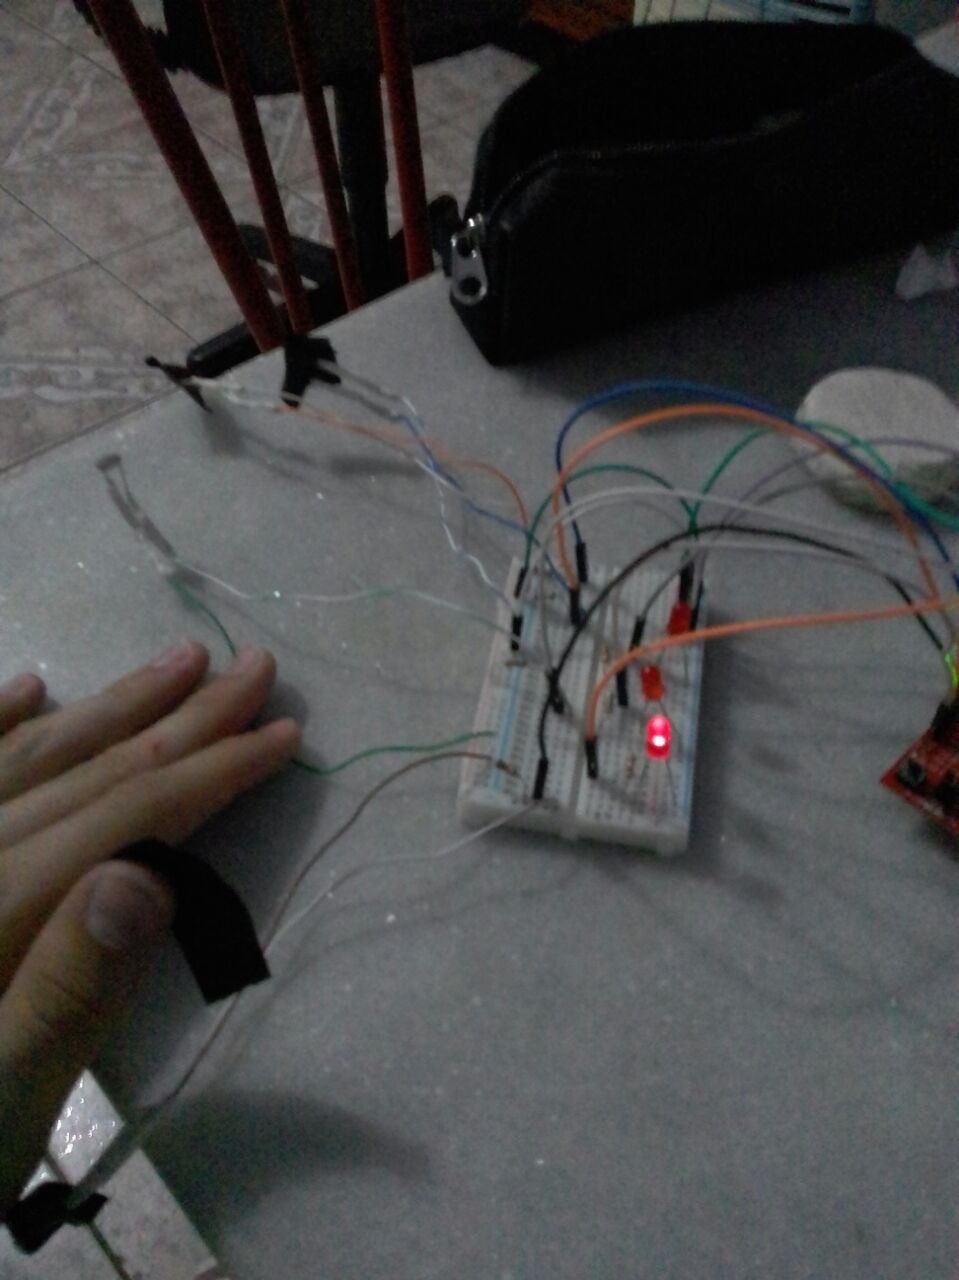
\includegraphics[scale=0.10]{resultado1.jpeg}
	%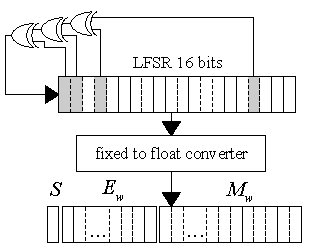
\includegraphics[scale=0.9]{figures/fig1_RNG.eps}
	\caption{Sensor Esquerdo sem fita-isolante, motor direito acionado - Representa��o com LEDs}
	\label{fig3}
\end{figure}


\begin{figure}[H]
	\centering
	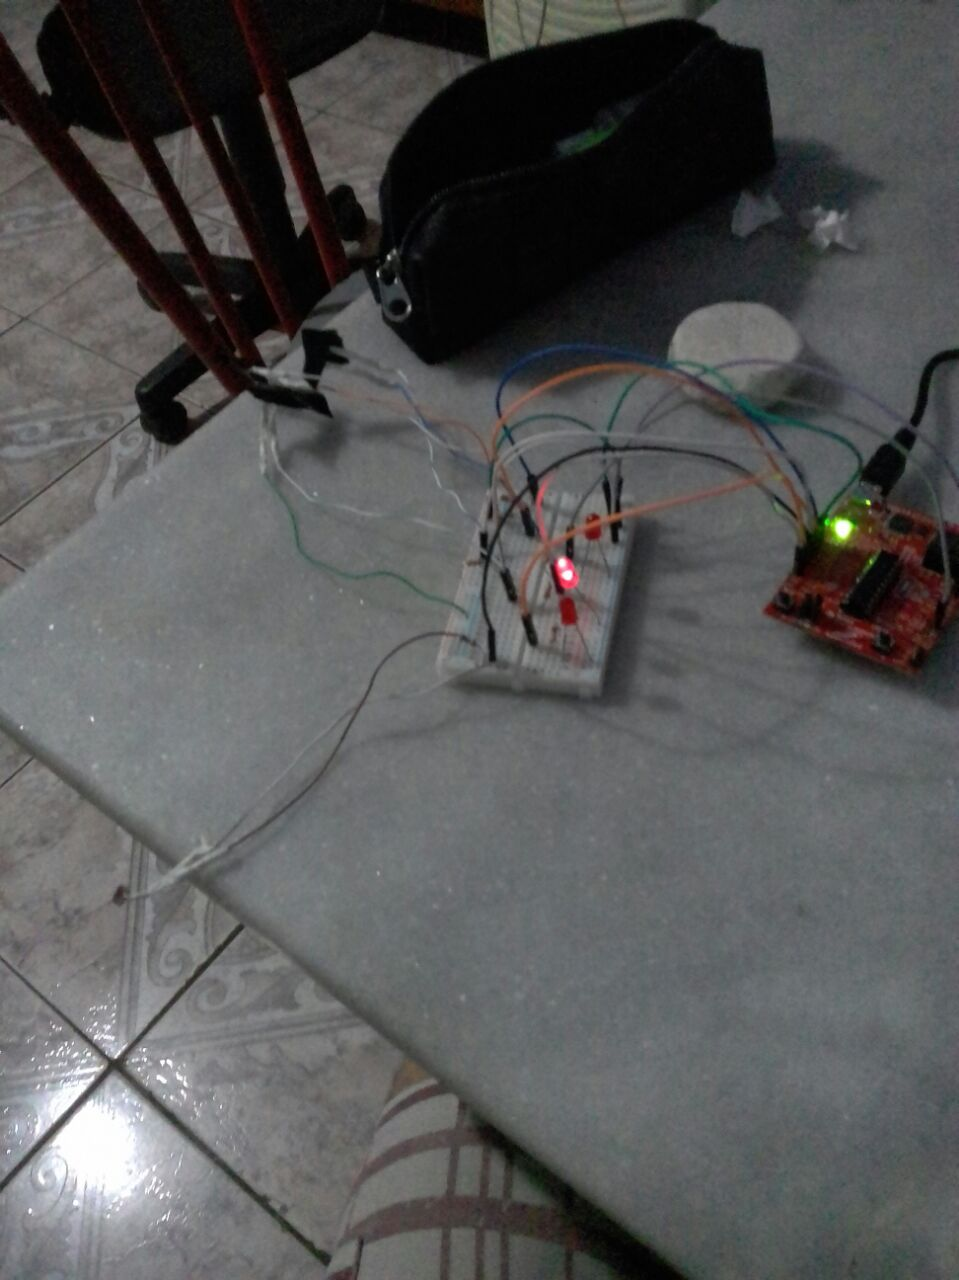
\includegraphics[scale=0.10]{resultado2.jpeg}
	%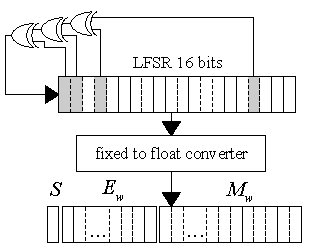
\includegraphics[scale=0.9]{figures/fig1_RNG.eps}
	\caption{Sensor Direito sem fita-isolante, motor direito acionado. O mesmo ocorre se o sensor traseiro � acionado (fica sem fita isolante) - Representa��o com LEDs}
	\label{fig4}
\end{figure}


\begin{figure}[H]
	\centering
	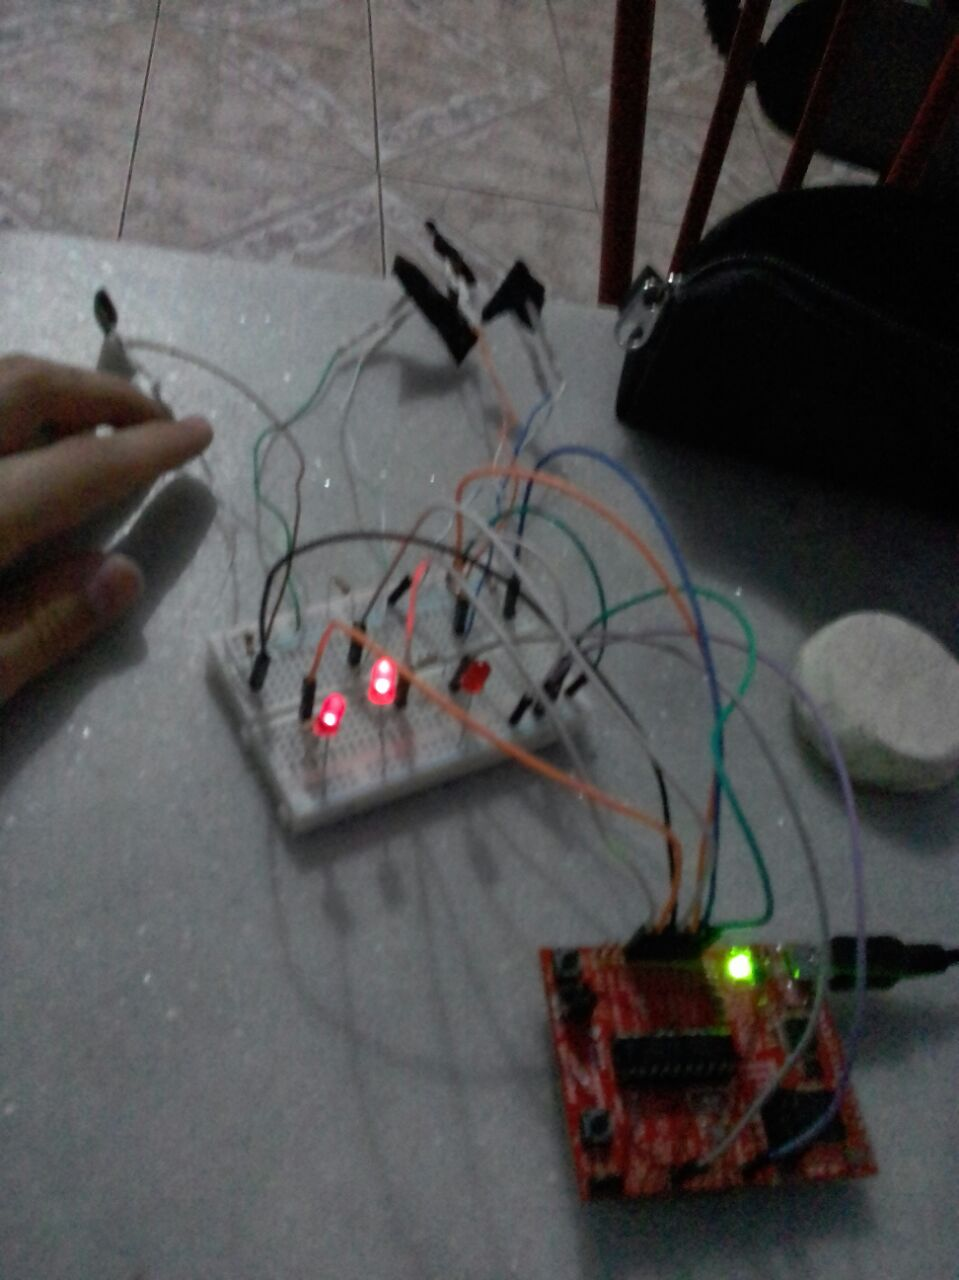
\includegraphics[scale=0.10]{resultado3.jpeg}
	%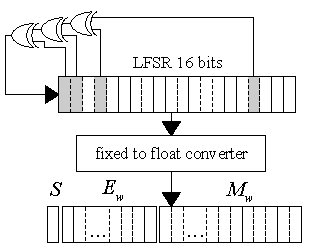
\includegraphics[scale=0.9]{figures/fig1_RNG.eps}
	\caption{Sensor Frente sem fita-isolante, motor direito e esquerdo acionado - Representa��o com LEDs}
	\label{fig5}
\end{figure}

\begin{figure}[H]
	\centering
	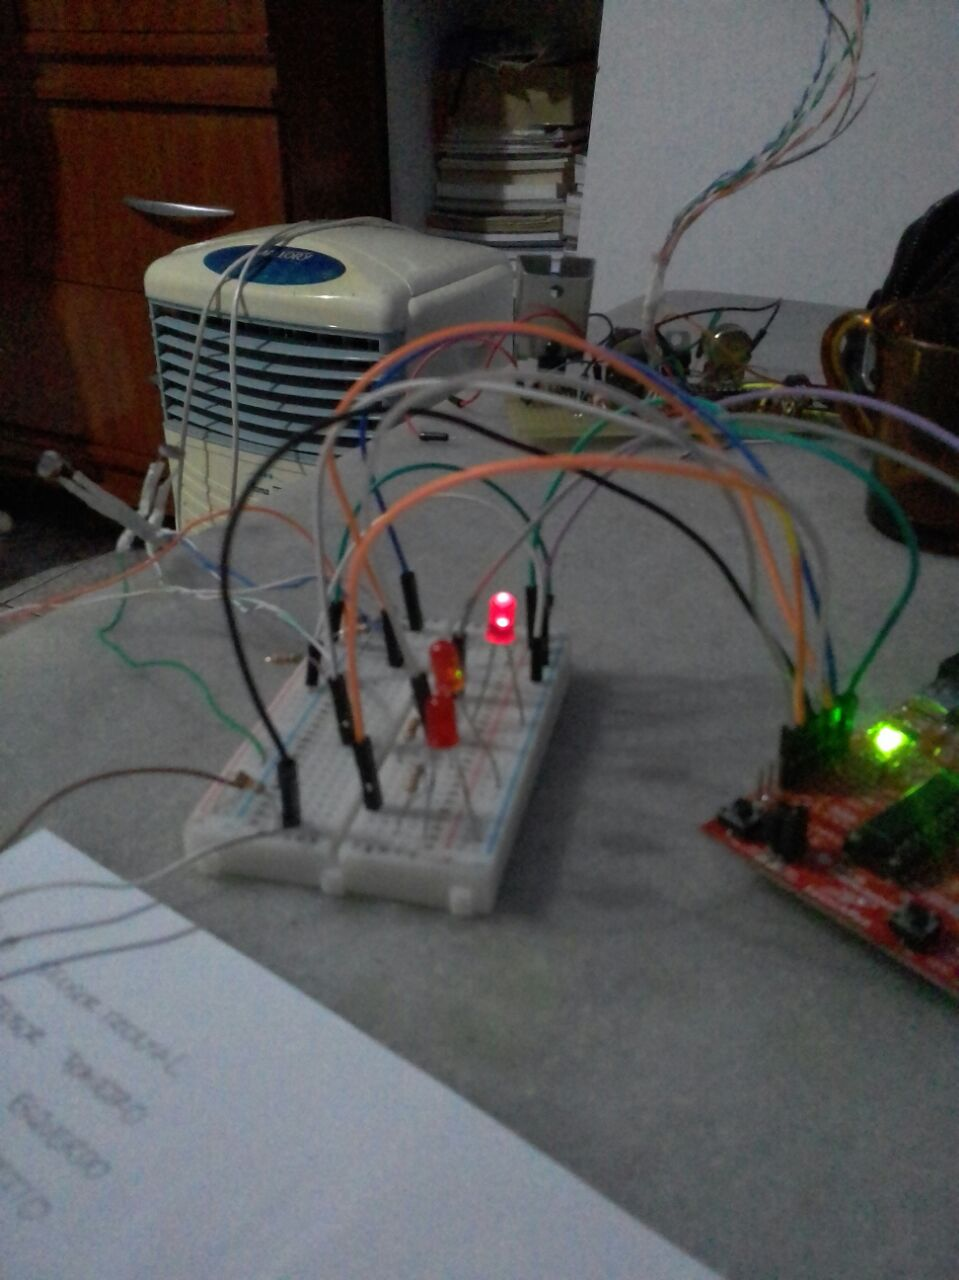
\includegraphics[scale=0.10]{resultado4.jpeg}
	%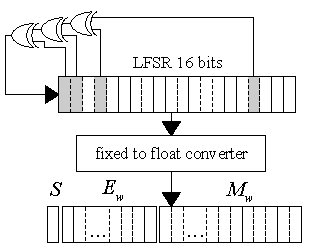
\includegraphics[scale=0.9]{figures/fig1_RNG.eps}
	\caption{Todos os Sensores Acionados, Arma disparada - Representa��o com LEDs}
	\label{fig6}
\end{figure}